\chapter{Design}
This chapter summarizes the overall design of our approach to generating textual medical reports for X-ray images. The problem consists of multiple independent parts we need to deal with. For each of them, we we will present the fundamentals of our solution, along with description of related problematics and decisions made.

\section{Our approach}
As we already mentioned in the Chapter \ref{sec:RelatedWork}, the overall solution for the final medical report generation model is based on the \citet{alfarghaly2021automated}. We have chosen this approach for multiple reasons. The main reasons to use this work as the backbone for our thesis are following:
\begin{enumerate}
	\item In the work the state-of-the-art GPT-2 model is utilized as the language model. This gave us a great opportunity as there was none Czech GPT-2 model available at the time this thesis began.
	\item The encoder is already fine-tuned to extract visual features for specific dataset.
	\item All solution source code is freely accessible on the github\footnote[1]{\url{https://github.com/omar-mohamed/GPT2-Chest-X-Ray-Report-Generation}}.
\end{enumerate}

As in most works for image captioning, the architecture is encoder-decoder based with an attention mechanism. The high-level solution architecture is depicted in Figure \hyperref[fig01:OmarArchitecutre]{2.1}.\\

The encoder part utilizes fine-tuned Chexnet\citep{rajpurkar2017chexnet} as its visual backbone. The Chexnet is a CNN Densenet121 model trained specifically for medical enviroment on the ChestX-ray14\citep{wang2017chestx} dataset predicting 14 distinct disease classes from the input chest X-ray images. Input images are resized to the $224 \times 224$ resolution as in the case of the original Chexnet model. Moreover, the encoder is further fine-tuned to predict 105 of the most common manual tags from the Indiana University chest X-ray dataset(see Chapter \ref{sec:IUDataset}) for the purpose of wider range of possible semantic features. The model thus produces two types of outputs - visual features from the base CNN model and class scores from the multi-label tag prediction.\\

In order to obtain semantic features from the predicted classes, each predicted class score is multiplied by its corresponding word2vec\citep{mikolov2013distributed} embedding, trained specifically on the biomedical texts, from the \citet{mcdonald2018deep} and resulting in the weighted embedding matrix. Both the embedding matrix and visual features are further passed to the language model as the context vectors for the self-attention mechanism.\\

Instead of the original English GPT-2 the original soluton used its smaller version distilGPT-2\footnote[2]{\url{https://huggingface.co/distilgpt2}}. The distilled version differs in the number of layers as it contains only a half of the layers compared to the original model and predicts only 512 tokens instead of 1024. Nevertheless, distilled versions of GPT-2 do not usually work well for languages other than English due to their reduced capacity. For these reasons, we use the original architecture of the GPT-2 for further fine-tuning. But, our fine-tuned model will predict 512 tokens as well as the distilGPT-2. During the medical report generation training, the maximal sequnce length is set to 200.\\
 
\begin{figure}[h]\centering
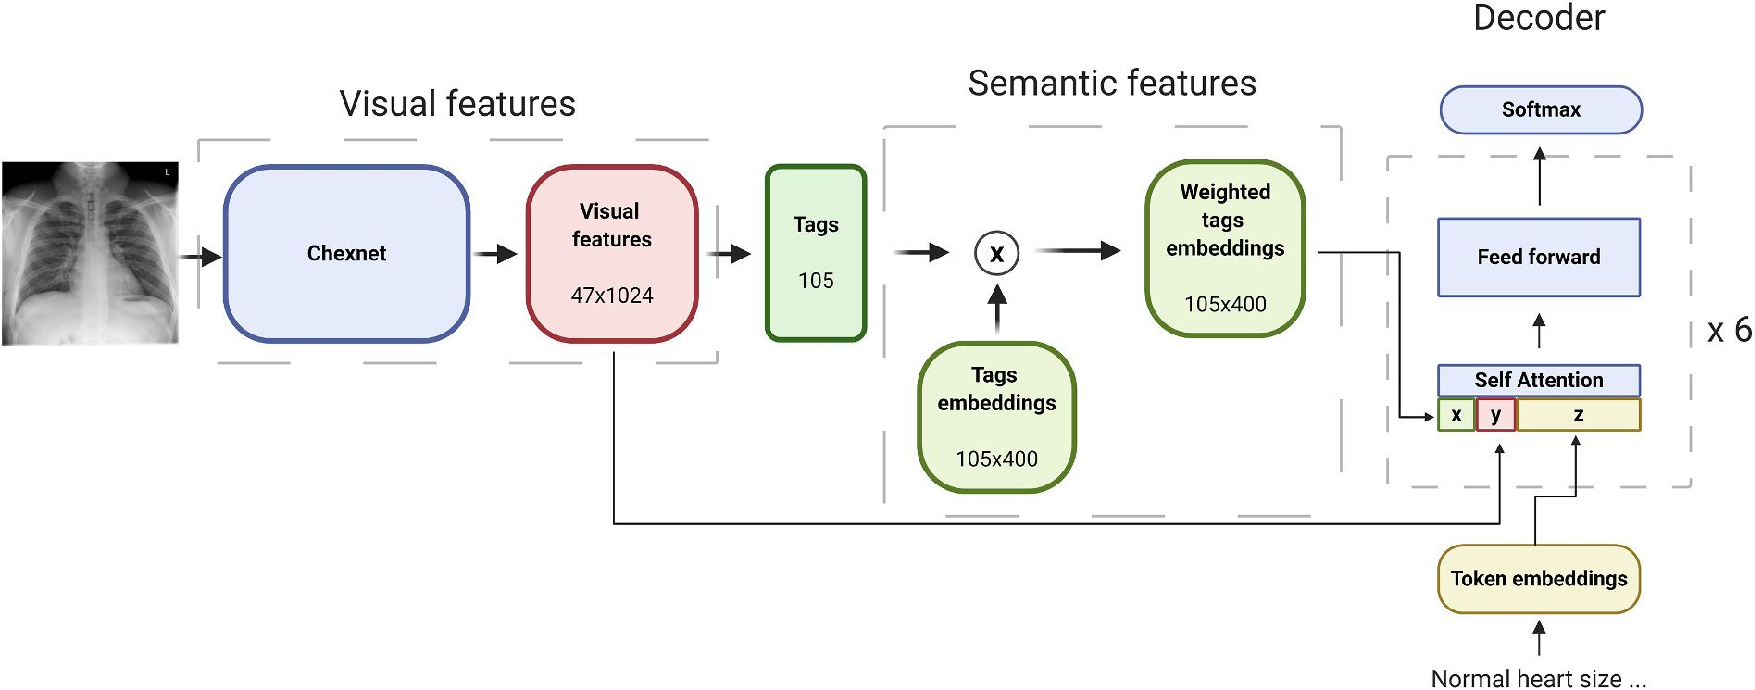
\includegraphics[width=145mm, height=57mm]{../img/OmarArchitecture}
\caption{Overall architecture used in our solution proposed in \citet{alfarghaly2021automated}.}
\label{fig01:OmarArchitecutre}
\end{figure}

\section{Czech GPT-2}
The aim of this work is to generate medical reports in the Czech language. In the previous parts, we decided to use the GPT-2 as the language model. However at the time of the beginning of this work, no Czech GPT-2 model was freely available and thus it was essentially necessary to create one. This section describes all the steps needed for fine-tuning the small English GPT-2 to the Czech language. Respectively, we train two versions of the Czech GPT-2 model. One trained on the general Czech textual data and one specialized specifically on Czech medical texts.

\subsection{Data}
\label{sec:gptData}
In this section we will describe the possible data applicable for training of both the general and medical Czech GPT-2 model together with the decision made about the final data selection and data cleaning.

\subsubsection{General}
For the training of general Czech GPT-2 we have a plenty of data options we can choose from. However, there are important properties of the data we need to sastisfy. As we are transfer learning from English to Czech language we need to have sufficiently large data, so we ensure the GPT-2 will learn properly syntactical and semantical information. Moreover, the data have to be also heterogeneous enough, so the model can capture different types of information and not just for example newspaper articles from a specific area. In order to create a good enough general model we need to meet these criteria.\\

Several different datasets were investigated and tested for the training of the general Czech GPT-2 model.
\paragraph*{Czech Wikipedia} ~\\
\indent The first data we used for training the model is the Czech~Wikipedia~dump\footnote[2]{\url{https://dumps.wikimedia.org/cswiki/latest/cswiki-latest-pages-articles.xml.bz2}}. After extraction, the total size of the dataset is approximately 800 MB of raw text. The advantages of this dataset are its easy accessibility and fairly clean data quality. On the other hand, the data are very homogeneous despite the various topics. Each article is written in the general descriptive style. Moreover the data themself are not large enough, the trained model made many both syntactical and semantical mistakes during the text generation.

\paragraph*{Balanced Czech National Corpus} ~\\
\indent Another possibility was to use a balanced version of the Czech National Corpus\citep{11234/1-4635} as the original is composed mainly of journalistic articles. The balanced version tries to equalize the amount of data from each category. These categories include \textit{journalism}, \textit{poetry}, \textit{prose}, \textit{educational literature} etc. The major advantage of this dataset is its purity, the texts are syntacticaly correct without any undesirable non-Czech elements and written in the standard Czech language. The dataset does not have any significant downsides and the trained model understood Czech language without any significant ailments. In total, the dataset is comprised of 3,3 GB of raw text.

\paragraph*{OSCAR} ~\\
\indent OSCAR, from the \citet{ortiz-suarez-etal-2020-monolingual}, is a huge deduplicated multilingual corpus created from the Common~Crawl~corpus\footnote[3]{\url{https://commoncrawl.org/}} providing data for 166 different languages and available directly in the huggingface datasets library\footnote[4]{\url{https://huggingface.co/datasets/oscar}}. It consists of the text scraped from websites of very different kinds and thus the data are heteregeneous enough. Moreover, its huge size, as the czech part of the dataset occupies a total of 24 GB of raw text, is another major benefit. On the other hand, because the data are automatically scraped, they carry a noise in them. Besides that, not negligible part of the text are in the non-standard Czech language as the data come from diverse web sources such as forums etc. Nevertheless, the disadvantages are outweighed by the huge size of the corpus and together with following filtering of the text:
\begin{enumerate}
	\item We take only text that are at least 1200 characters longs as these texts tend to be longer articles written in the standard Czech language instead of advertisements, incomple texts etc.
	\item Any text containing control character are filtered out, because the text contains generally undesirable content.
\end{enumerate}

\paragraph*{Conclusion} ~\\
\indent We analyzed various datasets along with their overall properties. Furthermore, the advantages and disadvantages of each were discussed. As a result, we have chosen the \textbf{OSCAR} dataset due to its size and heterogeneity. The \textbf{Wikipedia} is too small and homogeneous. On the other hand the \textbf{Balanced Czech National Corpus} is heterogeneous enough, however it is an almost order of magnitude smaller than \textbf{OSCAR}.

\subsubsection{Medical}
Since we have a trained general Czech GPT-2 model from the previous section that already understands a Czech language, the final fine-tuning for medical environment does not require that much data. We need to specialize the model to understand the mecial environment inherently. For this purpose, we use a subset of the UFAL~Medical~Corpus~v. 1.0\footnote[5]{\url{https://ufal.mff.cuni.cz/ufal\_medical\_corpus}}. These data are further filtered to remove any inappropriate characters, lines and redundant structures. As a result, the data contain a total of 100 MB of raw medical texts. The texts comprise of general medical descriptions, articles and package leaflets for medicines.

\subsection{Training}
In this part, we will describe the fine-tuning process of our Czech GPT-2 models. Both the general and the medical GPT-2 models will be trained using the same process. The solution is based on the \citet{guillou2020faster} article using specific fastai\footnote[6]{\url{https://www.fast.ai/}} library providing with powerfull tools using best practices aiming for training and fine-tuning neural network models. The reason why we used this article is that it has shown great results for transfer learning the English GPT-2 to another language in a short time againts traditional fine-tuning. The whole process comprises of several important parts, that we will describe in the subsequnet part of the text. Detailed information about the insides and experiments done are described in the following Chapters TODO.

\subsubsection*{Training tokenizer}
First thing that needs to be done in the whole training process is to train a tokenizer specifically for the Czech language. As in the case of original GPT-2 model, we use the same byte-level~byte-pair-encoding\footnote[7]{\url{https://huggingface.co/course/chapter6/5?fw=pt}} tokenizer dividing input text into tokens (a word or its part). Original size of the vocabulary is kept and set to 50257, as well as the original special token $<|$endoftext$|>$ as indication of the beginning/end of the sequence token and the pad token. The entire prepared datasets from Chapter \ref{sec:gptData} are used for the tokenizers training.

\subsubsection*{Initialization}
As we have indicated several times, for the GPT-2 model weights initialization we will use the weights from the original English GPT-2. However, we will do a modification of the initial word token embeddings.\\

For the word token embedding, we will compare what tokens have the English model tokenizer and our tokenizer in common. The embeddings of these tokens will remain unchanged, as they have been already trained on a large text corpus and they already carry information, even though they come from a completely different language. The rest of the tokens will be initialized using the mean value of the English word token embeddings.

\subsubsection*{Data preparation}
Another step in the process is to prepare the dataset into suitable structure for the training. Entire dataset is loaded and pre-tokenized in advance in order to reduce the data transfer time between CPU and GPU needed. After the pre-tokenization process, all texts are further passed passed to a specific language modeling data object, that is responsible for preparation and handling of training and validation data. All texts are concatenated, split by the defined sequnce length and formed into the batches. We use bach size of 16 as it is the maximum size we were able to fit into the GPU and sequence length of 512, because we need to have model correponding to the one used in \citet{alfarghaly2021automated} - distilGPT2 - as our main goal is to generate medical reports.\\

The batch size is one of the important hyper-parameters. In the following section we will discuss, how learning rates are determined and also that we will use higher learning rates. Nevertheless, in the \citet{smith2018disciplined} they recommend to use batch size as large as possible, because higher learning rates are regularization themself and therefore other regularizations can be reduced.

\subsubsection*{Finding optimal learning rate}
Fine-tuning is a very fragile process in terms of learning rates. Right choice of the learning rate is essential, if we choose a very small learning rate, the model will train slowly and will tend to overfitting. On the other hand, if we choose too high learning rate, the whole process can diverge and all the progress will be lost.\\

\citet{smith2017cyclical} came with a solution to this problem. Before the training itself, we do a pre-training run in which we are trying a wide range of learnings rates for which we monitor their behaviour. Starting from a very low learning rates up to the very high learning rates, for every mini-batch we try a current learning rate, collect the resulting loss and move to the next iteration with a little higher learning rate. In the end, we plot collected losses against the corresponding learning rates.\\

An illustration of the result of this process can be seen in the Figure \hyperref[fig02:lrFinder]{2.2}. The graph gives us an overview for which learning rates the model is still learning. General recommendation is to use a learning rate that is an order of magnitude less than the minimum as the minimum is very close to the moment of divergence. We can also see in the graph that the current implementation gives us several other significant points usable for training.

\begin{figure}[h]\centering
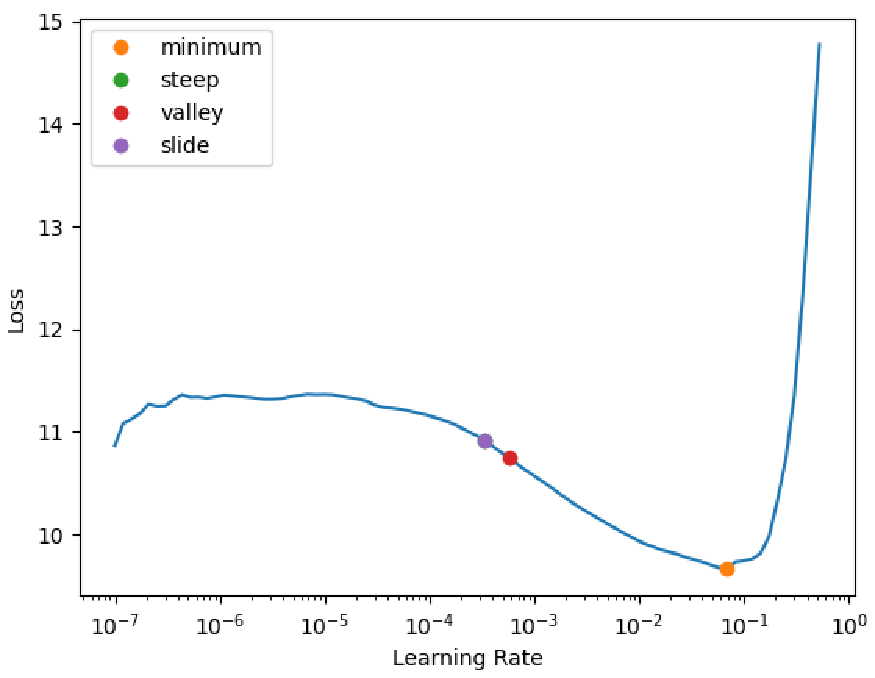
\includegraphics[width=130mm, height=101mm]{../img/lrFinder}
\caption{Learning finder output.}
\label{fig02:lrFinder}
The \textit{Learning rate} axis is in logarithmic scale.
\end{figure}

\subsubsection*{Training process}
We have prepared everything we need in the previous parts. However, we still have to describe the essence of our fine-tuning process. We will first describe the learning rate schedule. Fine-tuning or transfer learning is usually done using small learning rates with decay, so the general information in the already pre-trained weights are kept while the model is specialized to a selected task. The disadvantage of this method is the long training time. Instead, we use a different approach from \citet{smith2018disciplined} called "1cycle" policy that is parametrized by \textit{minimal} and \textit{maximal} learning rates. In the beginning we start with a \textit{minimal} learning rate and linearly increase it up to the \textit{maximum}. The second phase is then the opposite direction going down with cosine annealing, but instead of stopping at the \textit{minimum} the decrease continues down by several order of magnitudes lower as we can see in the Figure \hyperref[fig03:lrSchedule]{2.3}. \\

The intuition behind this policy is quite natural. In the beginning we start with a lower learning rates to find an optimal direction. As we are increasing the learning rate we are taking bigger steps this direction, skipping sharp local minima and preferring wide flat local minima area as shown in the \citet{smith2019super}. The rest of the training is intented for improvement inside this area. This allows us to use higher learninng rates and thus overall accelerate the entire training process. The \textit{maximal} learning rate should be chosen according to the previous section and the \textit{minimal} is defined as $ min = max / 25$ by default.\\

Another major part of the training are discriminative learning rates. This method has been proposed in the \citet{howard2018universal}. Instead of training all layers at once, we assign a different learning rates for each layer or a group of layers as each of them. This arises from the reasoning about what the different parts of the network are focusing on. Therefore, we split our model into 4 distict groups of layers and train each of them with different learning rate.\\

The fine-tuning process itself is divided into two parts: training the new head for the Czech language only and training the whole model at once. In the original article, they suggest gradual unfreezing approach, where they unfreeze one more layer each time and train for one epoch. However after numerous experiments, we observed that unfreezing of the whole model and running multiple epochs at once gives better results.

\begin{figure}[h]\centering
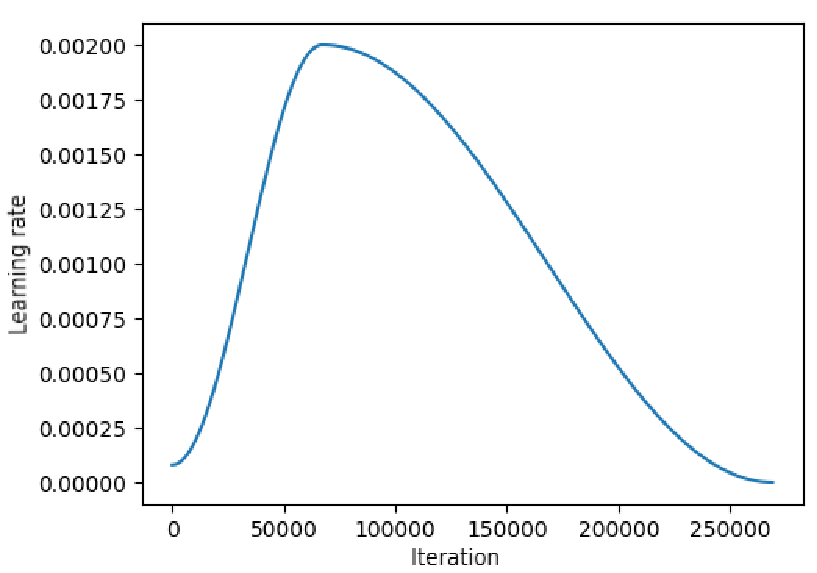
\includegraphics[width=130mm, height=91mm]{../img/lrSchedule}
\caption{Learning rate schedule for 1cycle policy training.}
\label{fig03:lrSchedule}
The graph depicts the learning rate throughout the entire training process.
\end{figure}

\section{Medical dataset translation}
For machine learning in general and NLP tasks especially, the data quality is the alpha and omega of the performance of the final model. Since, as we have already mentioned in the Chapter \ref{sec:CzechData}, we do not have any Czech data directly for the medical examinations of X-rays, to obtain Czech data we must arrange ourselves in a different way. One potential way is to create a new artificial dataset using machine translation of existing datasets. This section discusses the required steps to build a quality dataset using translation.

\subsection{Translator choice}
In the previous part of the text, specifically in the Chapter \ref{sec:Translators}, we already discussed all possibilities for automatic translation. Our final choice for the translator is the CUBBITT as it provides REST API unlimited in the number of requests and volume.

\subsection{Preprocessing}
\label{sec:DataPreprocessing}
The most important part of our machine translation process is the preprocessing of the input text. We already outlined in the Chapter \ref{sec:datasets} that the data contain some noise in them as we are dealing with reports in natural language. Moreover, we will use CUBBITT translator, that doest not perfom auto-correction itself and cannot translate some patterns at all as we described in the Chapter \ref{sec:Cubbitt}. For these purposes we incorporate preprocessing before the translation as it would be beneficial to have all texts in standardized form in order to firstly, help CUBBITT with translation to get the report correctly translated, and secondly to ensure that our model receives and process all the data in a indentical report format.\\

Our preprocessing pipeline encompasses of following procedures. Some of them are dealing with general CUBBITT issues and other with specifics of the medical data.

\subsubsection*{Line starts}
First of all we start with a very simple procedure. We analyze all lines of the report and delete all white characters common for all lines on both ends. The purpose of this modification is to standardize the report format, while preserving its structure.

\subsubsection*{Anonymous sequences}
Inasmuch as the whole datasets are anonymized due to the legal reasons and privacy protection, the reports contain \qq{anonymous sequences}, such as \qq{XXXX} or \qq{\underline{{ }{ }{ }{ }{ }}}, denoting places with original private information about patients. However, these sequences can be attached to surrounding words forming undesirable words. As we already said, the CUBBITT does not auto-correct its input automatically, so these inputs will not be handled in any special way and therefore not translated. For this reason, we separate these sequences to form independent words.

\subsubsection*{Units}
Subsequent form of correction that we perform is the separation of numbers and units attached to them. In addition, this also includes general cases, where the number and subsequent word are glued together, while keeping specific medical terms with a similar structure. This is associated with the following step, as the units will not be true-cased properly without this procedure.

\subsubsection*{True-casing}
The most imporant part of the whole preprocessing pipeline is true-casing of the input text. This adjustment is necessary for two essential reasons. CUBBITT has problems with translation of any uppercase texts in general. Capturing the true-case of a text is a complex problem requiring either a large statistical language dictionary or a trained model in order to properly determine the case.\\

As medical reports are very specific area, the existing solutions for general text true-casing is inapplicable. Medical reports contain a lot of abbreviations and acronyms, which can be often confused with ordinary english words. Training the model for medical true-casing requires even more specific data for a certain domain, because in different contexts the common words can be treated differently. Moreover, obtaining flawless data to cover the entire specific domain is a challenging task. For these reasons, we chose the way of a statistical dictionary. Before the translation of the dataset begins, we create a statistical dictionary from the whole dataset containing the most often used form of every word. We also count with some exceptions, such as headings, that in some datasets can be in uppercase only.\\

Using the created dictionary, we deal with all uppercase words to assign them the proper form. The results of the true-casing preprocessing are demonstrated in the following examples:
\begin{itemize}
	\item (1a) \qq{EXAMINATION: CHEST (PORTABLE AP)} $\rightarrow$ \\ \phantom{(1a)} \qq{PŘEZKOUŠENÍ: CHEST (PORTABLE AP)}
	\item (1b) \qq{Examination: Chest (portable AP)} $\rightarrow$ \\ \phantom{(1b)} \qq{Vyšetření: Hrudník (přenosný~AP)}
	\item (2a) \qq{SMALL RIGHT PLEURAL ABNORMALITY} $\rightarrow$ \\ \phantom{(2a)} \qq{MALÉ PRÁVO PLEURÁLNÍ ABNORMALITY}
	\item (2b) \qq{Small right pleural abnormality} $\rightarrow$ \\ \phantom{(2b)} \qq{Malá pravá pleurální abnormalita}
\end{itemize}

\subsubsection*{Paragraphs structure}
In some of the medical reports the section headings and corresponding texts do not begin on the same lines. We adjust these situations to a form where each heading and the text belonging to it always starts on the same line, for two reasons. Firstly, we want to normalize the report structure in general and secondly, we want to move the section content as close as possible to the heading, so the translator and even the final model have the context close to each other.

\subsubsection*{Capitalization}
Another part of the preprocessing pipeline is a simple capitalization of each heading and each sentence in the report. This text capitalization process helps CUBBITT not only in the case of medical data, but in general during the translation process of some texts to better understand the boundaries between sentences.

\subsubsection*{Time}
One of the patterns that CUBBITT doest not recognize nor auto-corrects itself in general are times. This applies both, to the specification of hours and minutes, and to the  part of the day specification. If any of these parts are incorrectly formatted, the time will we translated incorrectly or not translated at all, and thus we would lose some information or it could damage the fluency of the translated text. For these reasons, we apply preprocessing to normalize all times. We can see the difference in the following examples:
\begin{itemize}
	\item \qq{Chest radiograph at 1045PM} $\rightarrow$ \qq{Rentgen hrudníku v 1045PM}
	\item \qq{Chest radiograph at 10:45 PM} $\rightarrow$ \qq{Rentgen hrudníku ve 22:45}
\end{itemize}

\subsubsection*{White spaces}
After all previous procedures, we apply one last very simple final modification, namely, we squash all the whitespace characters inside each line into a single space, while maintaining the format from the very first preprocessing step described above. This step is performed only for normalization purposes.

\subsubsection*{Lowercasing}
The last preprocessing procedure we will mention is lowercasing of the whole text followed by capitalizing the first word of each sentence. This is a separate procedure that was used in the earlier phases of elaboration of this work as CUBBITT has problem with uppercased word as we already mentioned.















